



Die grundlegende Idee bestand darin eine Zeit-Frequenz-Analyse mit Wavelets zu machen. Diese wird dann verwendet, um die Signale nach belieben zu manipulieren. Um die Rechenzeit zu minimieren, sollte ein mglichst schneller Algorhytmus verwendet werden. Dafür bietet sich die Multiskalenanalyse, mit ihrem schnellen Rechenalgorhytmus an. Jedoch ist jener so konipiert, keine redundante Daten zu erzeugen. Das mit der Multiskalenanalyse, mit ihrer $2^{n}$-fachen Fensterung, nur die Oktaven eines Siganles ersichtlich sind, ist für diese Vorhaben nicht von Vorteil. Besonders da die Tonleiter aus 12 Halbtönen in einer Oktave besteht. Dabei sind die Halbtöne mit dem Faktor $2^{\frac{1}{12}}$ in der Oktave verteilt. Die nebeneinanderliegenden Halbtöne sind dadurch für eine Multiskalenanalyse unsichtbar. \\
In diesem Kapitel wollen wir eine Methode erzeugen, mit deren Hilfe es möglich ist, einzelne Halbtöne in einer Oktave zu unterscheiden. Dafür sollen Frames und die Multiskalenanalyse verwendet werden.




\subsection{Framing}
Die normale Multiskalenanalyse verwendet nur Orthonormierte Basen. Weshalb sie auch keine redundante Daten erzeugt. Zu Analysezwecken, würde es sich lohnen mehr von diesen Basen zu erzeugen. Die zusätzlich entstandenen Informationen können dann zur Analyse verwendet werden. Fügen wir mehr Basen zu unserem Signale hinzu ensteht ein Frame. Genauere Abhandlungen über Frames sin im Kapitel\ref{chapter:geometrie} unter \ref{subsetion:skript:frames:framesinrn} zu finden. Um sinvolle Frames zu gestalten wird die Problematik noch einmal genauer angeschaut.\\

Wir möchten ein Signal mit der Multiskalenanalyse so bearbeiten, dass wir die einzelnen Halbtöne in einer Oktave untersuchen können. Die Multiskalenanalyse liefert uns jedoch nur Resultate im Zweierlogarhytmus. Die $2^{n}$-fache Fensterung der Multiskalenanalyse ensteht durch die verwendung von orthogonalen Basen. Folglich sollte man doch einfach die Basen verändern.\\

Fügt man nun mehr Basen zu unserem Frame hinzu, können wir mit der Multiskalenanalyse Zwischenschritte in den Oktaven erzeugen. Das heisst, fügt man 12 linear unabhängige Basen zu einem Frame hinzu. Sollte man nach einer Multiskalenanalyse des Frames, 12 Schritte pro Oktave bekommen. Nun möchte man mit dem Frame Töne erkennen. Deshalb ist es nur sinnvoll mindestens 12 Basen zu verwenden. So wird die die Anzahl Basen $k$ mit
\[ 2^{n} \cdot 12 = k \]
definiert.\\
Um eine neue Basis für ein Frame zu erzeugen, wird das zu analysierende Signal neu gesamplet. Wobei jedes neue Sampling einer neuen Basis entspricht. Die erste Samplerate, die auf das Signal angewendet wird, ist die Grundbasis $f_{g}$. Von der Grundbasis aus werden Anzahl $k$ Basen hinzugefügt.
\[fs_{n}=f_{g}\cdot2^{\frac{n}{k}}\]

Nach dem Samplingtheorem ist es dabei sinnvoll die Samplefrequenzen zu vergrössern und nicht zu verkleinern.
\[ \frac{f_{\text{sampling}}}{f_{\text{Signal}}} \geq 2\]
Damit kann garantiert werden, dass kein Datenverlust oder Aliasing auftritt. Es empfielt sich ohnehin genügend Abstand zwischen Sampling- und Signlfrequenz zu lassen.\\

Da die Tonleiter nicht willkürliche Frequenzen abdecken, wird auch die Grundbasis der Frames auf die Tonleiter festgelegt. Dabei bietet sich der Kammerton $\text{a}^{1}$ auch A4 genannt an. Dieser ist mit 440 \text{[Hz]} definiert.\\




Hierzu ein praktisches Beispiel zu den Sampelfrequenzen. Folgende Werte werden gegeben:
\begin{itemize}
	\item Samplefrequenz $f_{g}=440$\text{[Hz]}
	\item Anzahl Basen $k=12$
\end{itemize}	

\[
fs
=
 \begin{pmatrix}
fs_{0}\\[1mm]
fs_{1}\\[1mm]
fs_{2}\\[1mm]
fs_{3}\\[1mm]
fs_{4}\\[1mm]
fs_{5}\\[1mm]
fs_{6}\\[1mm]
fs_{7}\\[1mm]
fs_{8}\\[1mm]
fs_{9}\\[1mm]
fs_{10}\\[1mm]
fs_{11}\\[1mm]
\end{pmatrix}
=
\begin{pmatrix}
440\cdot2^{\frac{0}{12}}\\[0.5mm]
440\cdot2^{\frac{1}{12}}\\[0.5mm]
440\cdot2^{\frac{2}{12}}\\[0.5mm]
440\cdot2^{\frac{3}{12}}\\[0.5mm]
440\cdot2^{\frac{4}{12}}\\[0.5mm]
440\cdot2^{\frac{5}{12}}\\[0.5mm]
440\cdot2^{\frac{6}{12}}\\[0.5mm]
440\cdot2^{\frac{7}{12}}\\[0.5mm]
440\cdot2^{\frac{8}{12}}\\[0.5mm]
440\cdot2^{\frac{9}{12}}\\[0.5mm]
440\cdot2^{\frac{10}{12}}\\[0.5mm]
440\cdot2^{\frac{11}{12}}\\[0.5mm]
\end{pmatrix}
 \text{[Hz]}
 \approx
 \begin{pmatrix}
 440\\[1mm]
466.164\\[1mm]
493.883\\[1mm]
523.251\\[1mm]
554.365\\[1mm]
587.330\\[1mm]
622.254\\[1mm]
659.255\\[1mm]
698.456\\[1mm]
739.989\\[1mm]
783.991\\[1mm]
830.609\\[1mm]
 \end{pmatrix}
 \text{[Hz]} 
\]
In dem Vektor $fs$ sind die Samplefrequenzen für das Frame enthalten. Damit können die dazughörigen Sampleintervalle berechnet werden. Um die  Signallänge von der Sampling Frequenz zu entkoppeln werden die Elemente von $fs$ als auf Samples pro Sekunde normiert.  
\[fs = \frac{\text{Samples}}{\text{Sekunden}}\]
Das Ziel ist es ein Frame zu erstellen, dessen Zeilen aus dem verschieden gesampleten Signal besteht. Die Signaldauer $T_{s}$ wird dabei mit der Anzahl Samples pro Sekunde Multipliert um damit den Kehrwert der Zeit $T$ zweischen den Samples zu erlangen.
\[T_{i}=\frac{1}{fs_{n}\cdot T_{s}}\]

Der Index $T_{i}\in[t_{0},t_{1},...,t_{k}]$ steht dabei für alle Diskrete Zeitwerte die für ein Sampling mit den $k$ Basen verwendet werden.
\[
\mathcal{T}
=
\begin{pmatrix}
\vdots\\
\sum_{n=-\infty}^{+\infty} \delta(t - nt_{i+1})\\
\sum_{n=-\infty}^{+\infty} \delta(t - nt_{i+2})\\
\sum_{n=-\infty}^{+\infty} \delta(t - nt_{i+3})\\
\vdots\\
\end{pmatrix}
\cdot x(t)
\]
Auf dieses Frame wird dann eine Multiskalenanalyse angwendet. In dem Frame gibt es verschieden viele abgetastete Werte in den einzelnen Zeilen da $T_{i}$ durch die höheren Frequenzen quantitative mehr Elemente dazubekommt. Die wenigsten Elemente findet man dabei in der ersten Zeile des Frames. Diese wird verwendet um die Anzahl Levels der msa zu bestimmen. 
\[level = \left\lfloor\log_2\left(\mathtt{
	\frac{\mathcal{T}\_\text{min\_len}}{\text{filter\_len -1}}}\right)\right\rfloor
\]
Mit Level0 wird dabei auf das oberste Level referenziert welches die kleinste Frequenzteiung erfährt. Die Levels laufen also reziprok zu den Basen welche von unten nach oben benannt sind. Um dies besser zu Ilustrieren sind die Anzahl und Positionen in dem Bild \ref{fig:frame_konst} konzeptionell abgebildet. Man ging dabei von der Ursprungsbasis von 55 Samples aus. Es wurde dann mit sechs unterteilungen also $k=6$ ein Frame gebaut welches dann über vier Levels dargstellt ist. In der Grafik \ref{fig:frame_konst} ist die Struktur der einzelnen Vektoren, deren Anzahl von Datenpunkten sowie derigen verschiebung gut ersichtlich. \\

\subsubsection{Stacking Frame} 
Das Resultat der msa liefert uns $k\cdot \text{Anz. Level}$ Vektoren zurück welche alle eine unterschiedliche Länge besitzen. Um sie sinnvoll zu Sortieren beginnt man mit der Tiefsten Basis auf dem höchsten Level. Die gleichwertigen Level werden dann übereinander gestapelt von der kleinsten Basis zur grössten. Dann kommt das nächste Level. Mit dieser Struktur hat man die besten Resultate ohne eingriffe in die eigentlichen Werte vorzunehmen. 


\begin{figure}[h]
	\centering
	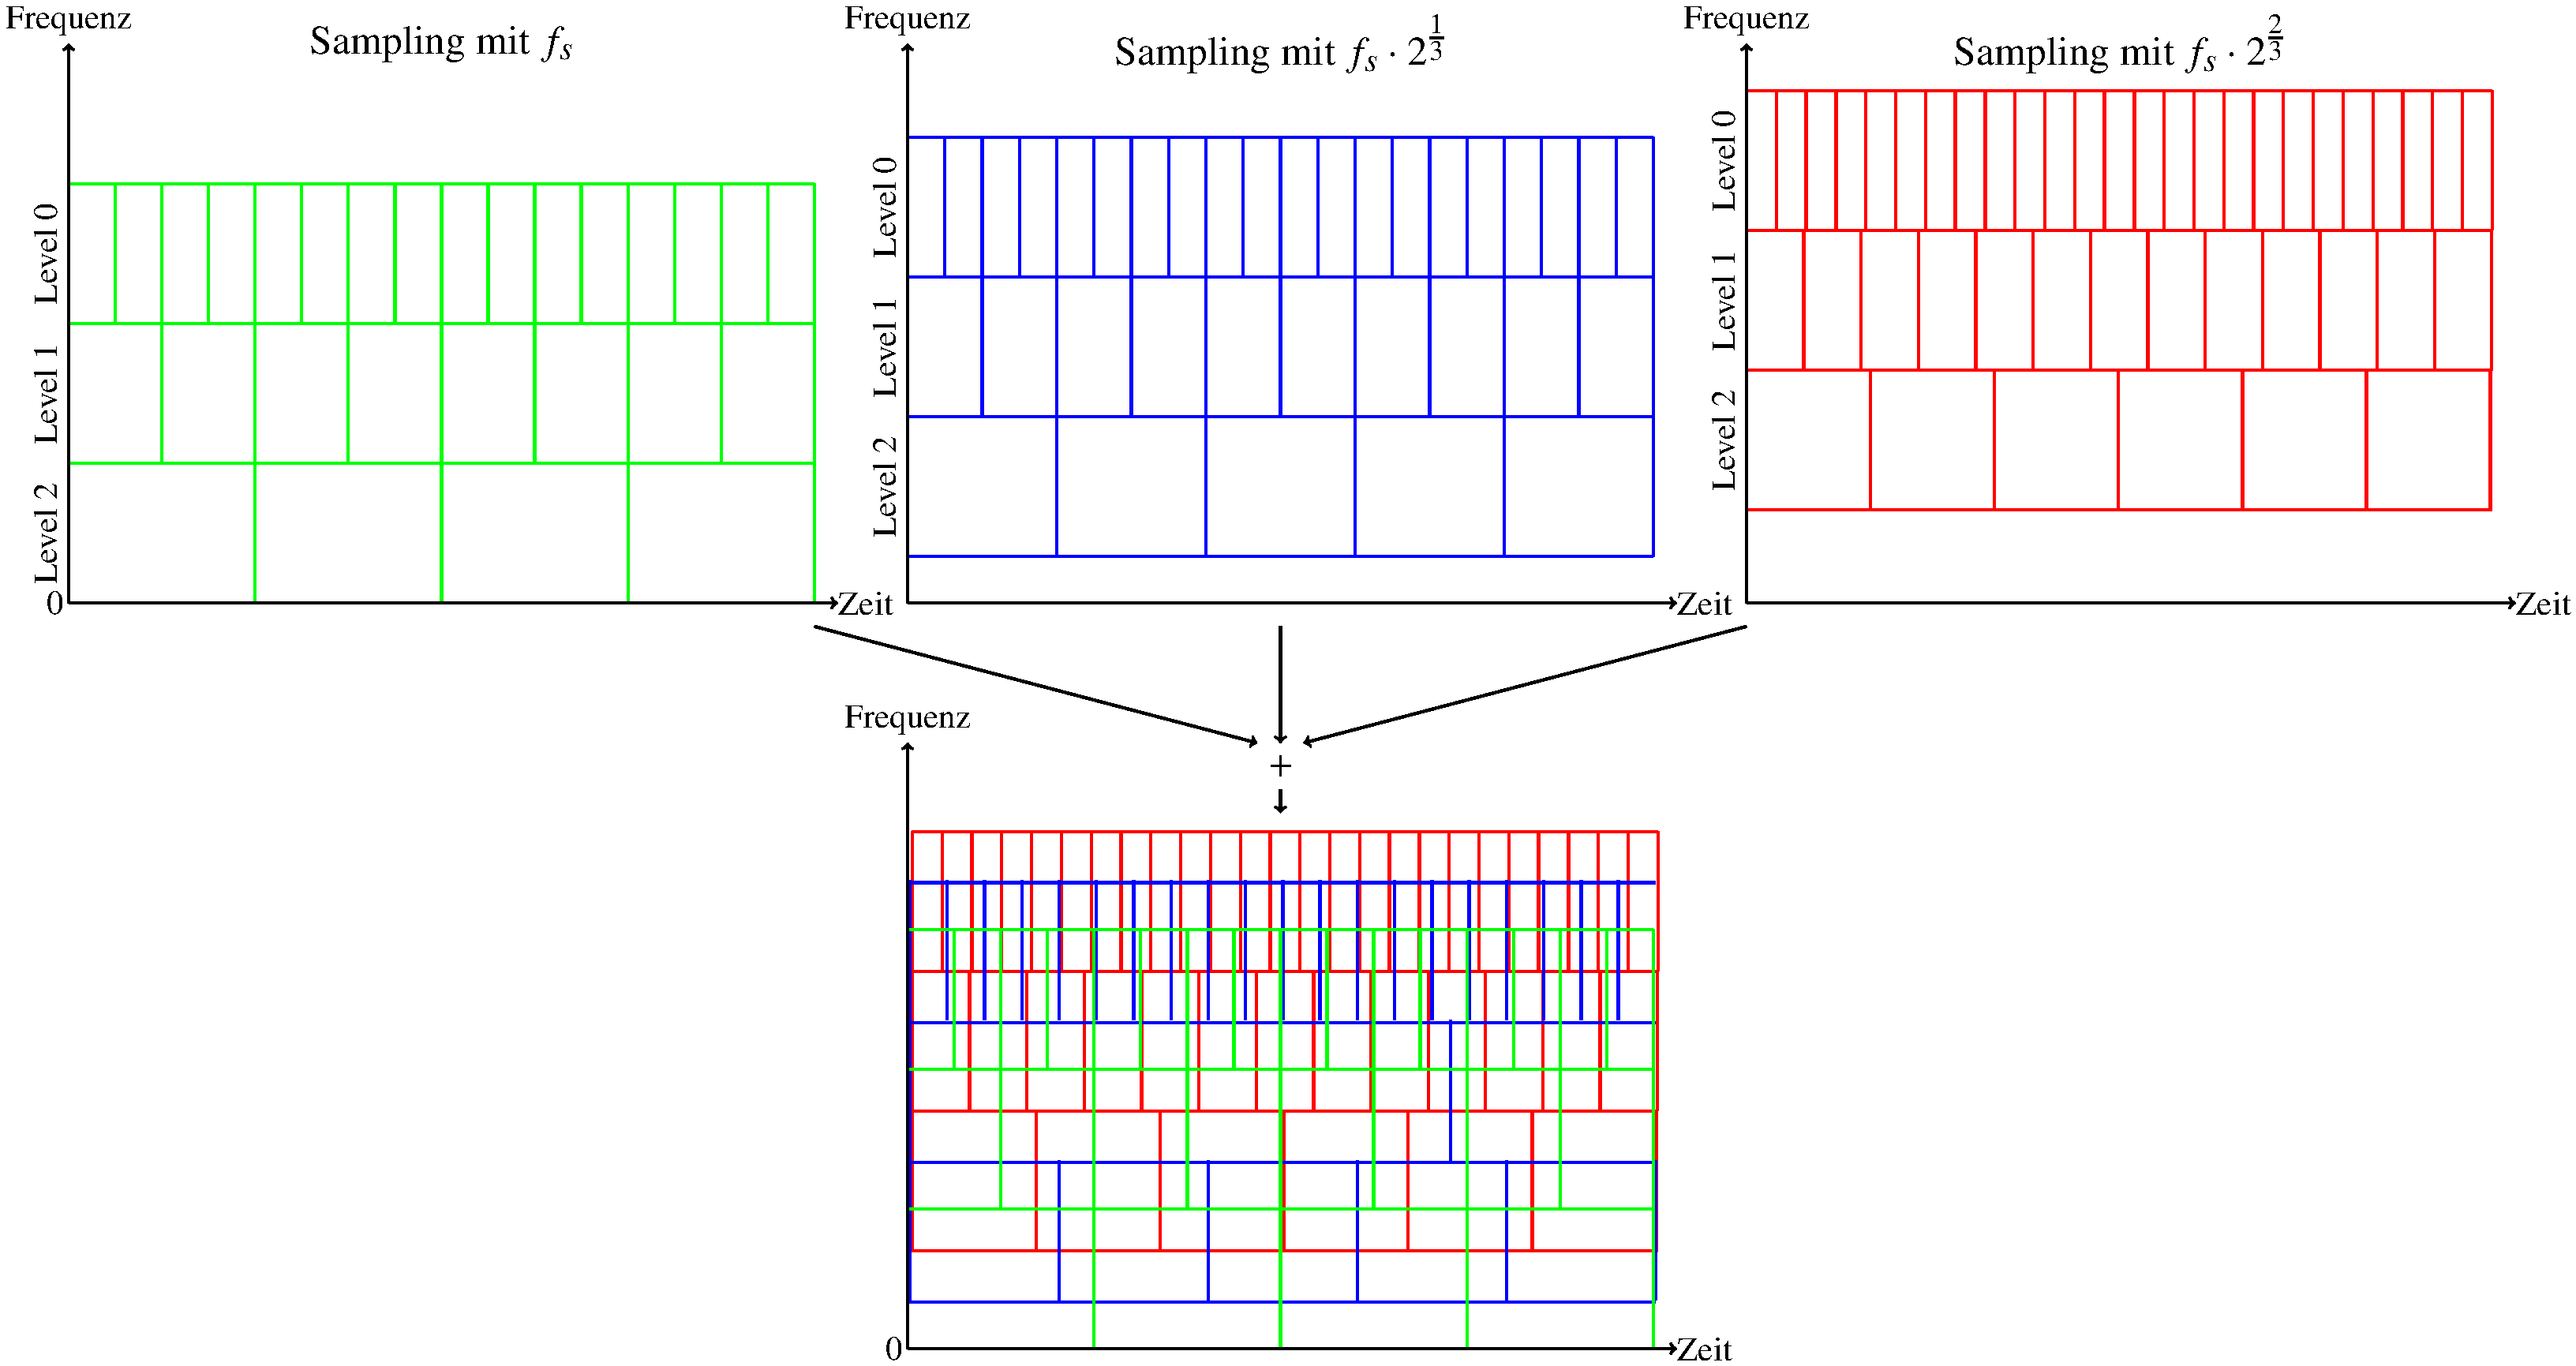
\includegraphics[width=\linewidth]{papers/autotune/sections/frames/images/frame/msa.pdf}
	\caption{Frame-Multiskalenanalyse mit 6 Basen und 4 Level gezeigt}\label{fig:frame_konst}
\end{figure}%

\subsubsection{Overlaying Frame}
Bla
\begin{figure}[h]
	\centering
	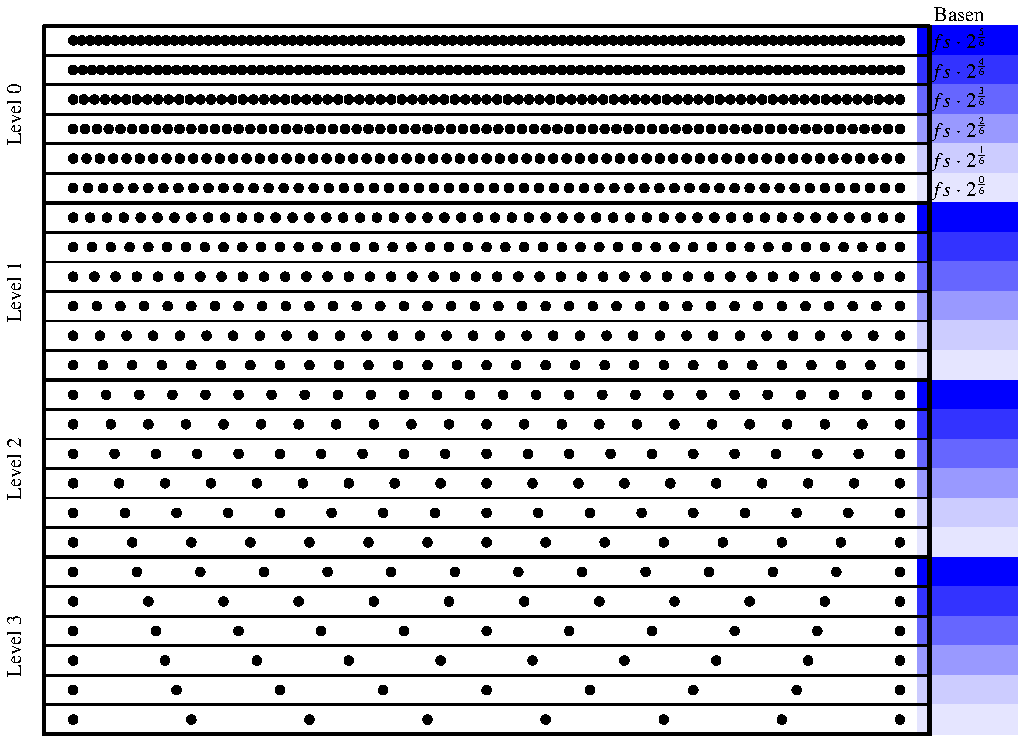
\includegraphics[width=\linewidth]{papers/autotune/sections/frames/images/msa/msa.pdf}
	\caption{Frame-Multiskalenanalyse mit 6 Basen und 4 Level gezeigt}\label{fig:frame_konst}
\end{figure}%


Die gleiche Methodik wie in Grafik \ref{fig:frame_konst} wurde für die anschliessenden Frame-Multiskalenanalysen verwendet.


\subsection{Analyse mit Frames}
In diesem Unterkapitel wird beschrieben welchen ablauf gewählt wurde um eine Analyse eines Testsignales durchzuführen.\\
Zuerst wurde ein Testsignal $x(t)$ erstellt. In der Grafik \ref{fig:frame-testsig} ist $x(t)$ abgebildet. Das Signal $x(t)$ besteht aus fünf verschiedenen Sinusschwingungen die aneinander gekoppelt wurden. Dazu eine kurze Beschreibung welche Frequenzen im dem Signal erhalten sind:\\
Die ersten zwei Ausschwenker schwingen über die dauer von jeweils $100$\text{ms}, mit der Frequenz 110 \text{[Hz]}. \\
Der dritte Ausschwenker schwingt $100$\text{[ms]} mit $220\cdot 2^{\frac{1}{12}}$\text{[Hz]}, folgend auf einen $100$\text{[ms]} Ausschwenker mit einer Frequenz von $220\cdot 2^{\frac{2}{12}}$ \text{[Hz]}. \\
Der letzte Block beginnt mit $220\cdot 2^{\frac{2}{12}}$\text{[Hz]} über eine dauer von $100$\text{[ms]} bis die Amplitude $a=1$ erreicht ist. Danach wechselt das Signal fliessend auf $220\cdot 2^{\frac{5}{12}}$\text{[Hz]} für $100$\text{[ms]} und endet mit $220\cdot 2^{\frac{6}{12}}$\text{[Hz]}. Die gesamte Signaldauer ist genau eine Sekunde lang. \\



In der Grafik \ref{fig:Frame-Analyse} wird eine Frame-msa und eine cwt-Analyse des gleichen Testsignales\ref{fig:frame-testsig} nebeneinander gestellt. Die Frame-msa wird dabei nur im Absolutwert dargestellt da so die Resultate noch eindeutiger sind. Im vergleich können nun die Unterschiede erkannt werden. Die Frame-msa hat deutliche Peak- und Nullstellen an Orten wo die cwt keine solche schwankungen aufweist. 
\begin{figure}[!ht]
	\centering
	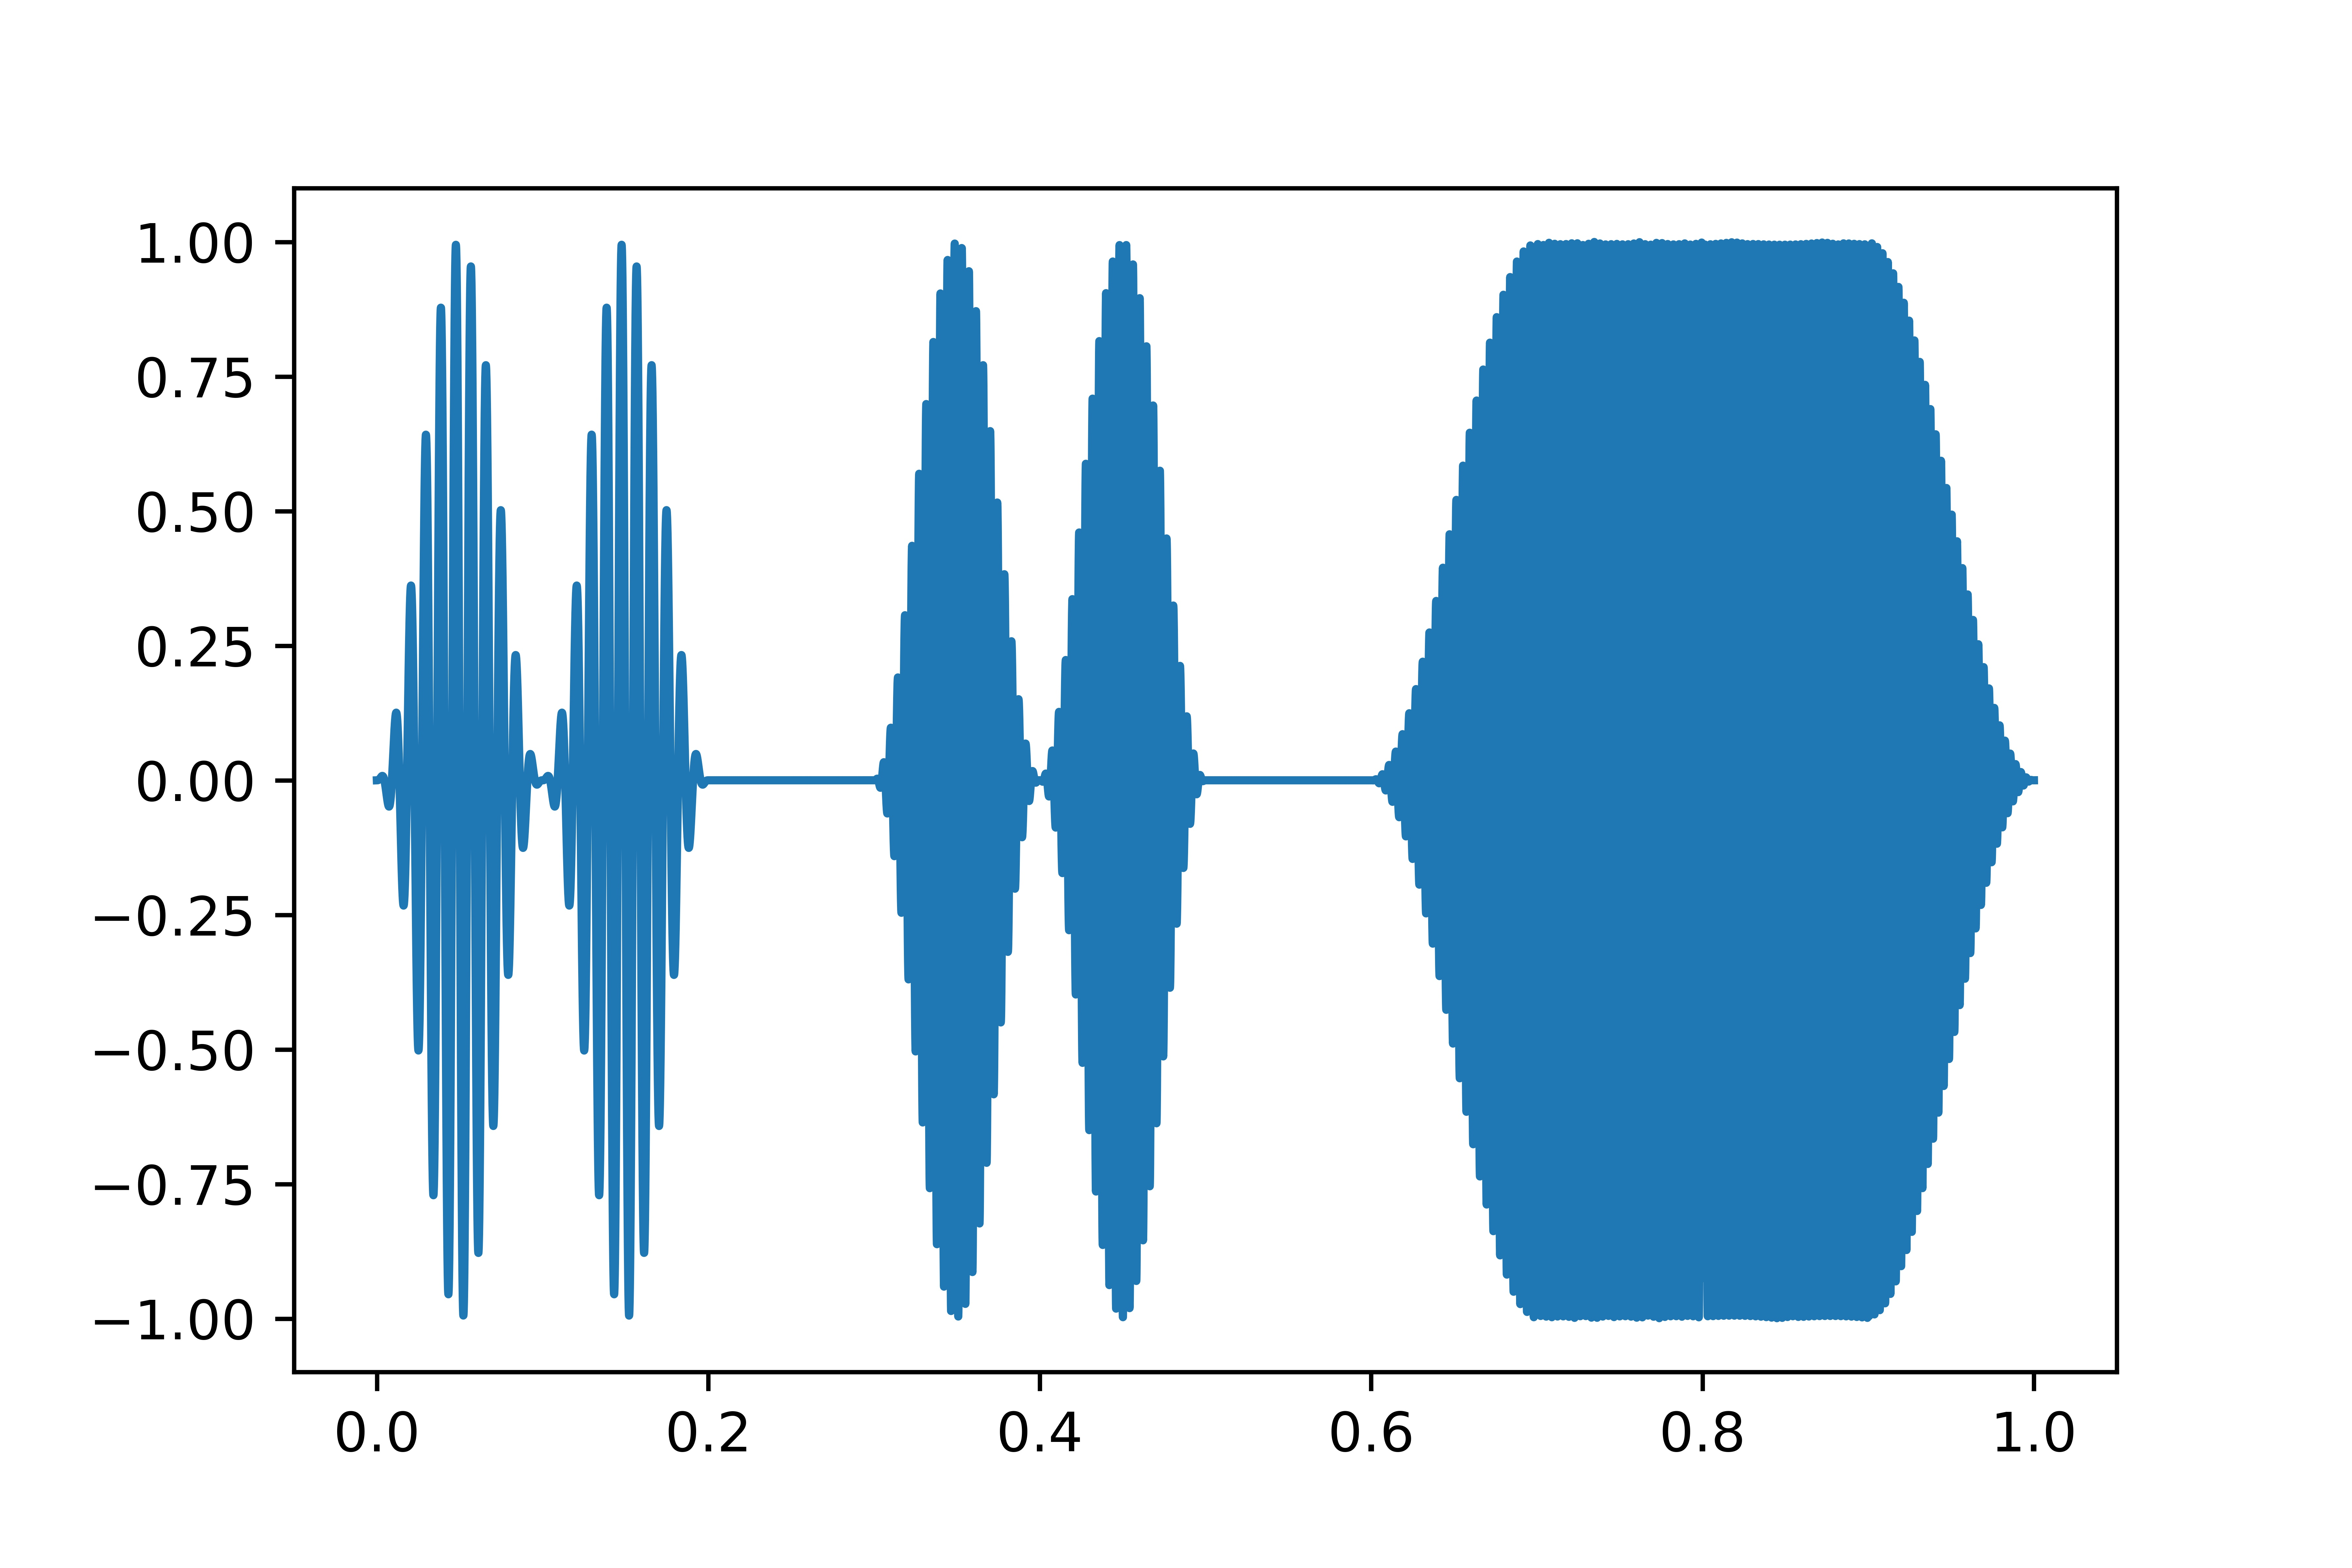
\includegraphics[width=0.9\linewidth]{papers/autotune/sections/frames/images/testsig.jpg}
	\captionof{figure}{Testsignal}\label{fig:frame-testsig}
	\begin{tabularx}{\columnwidth}{XX}
		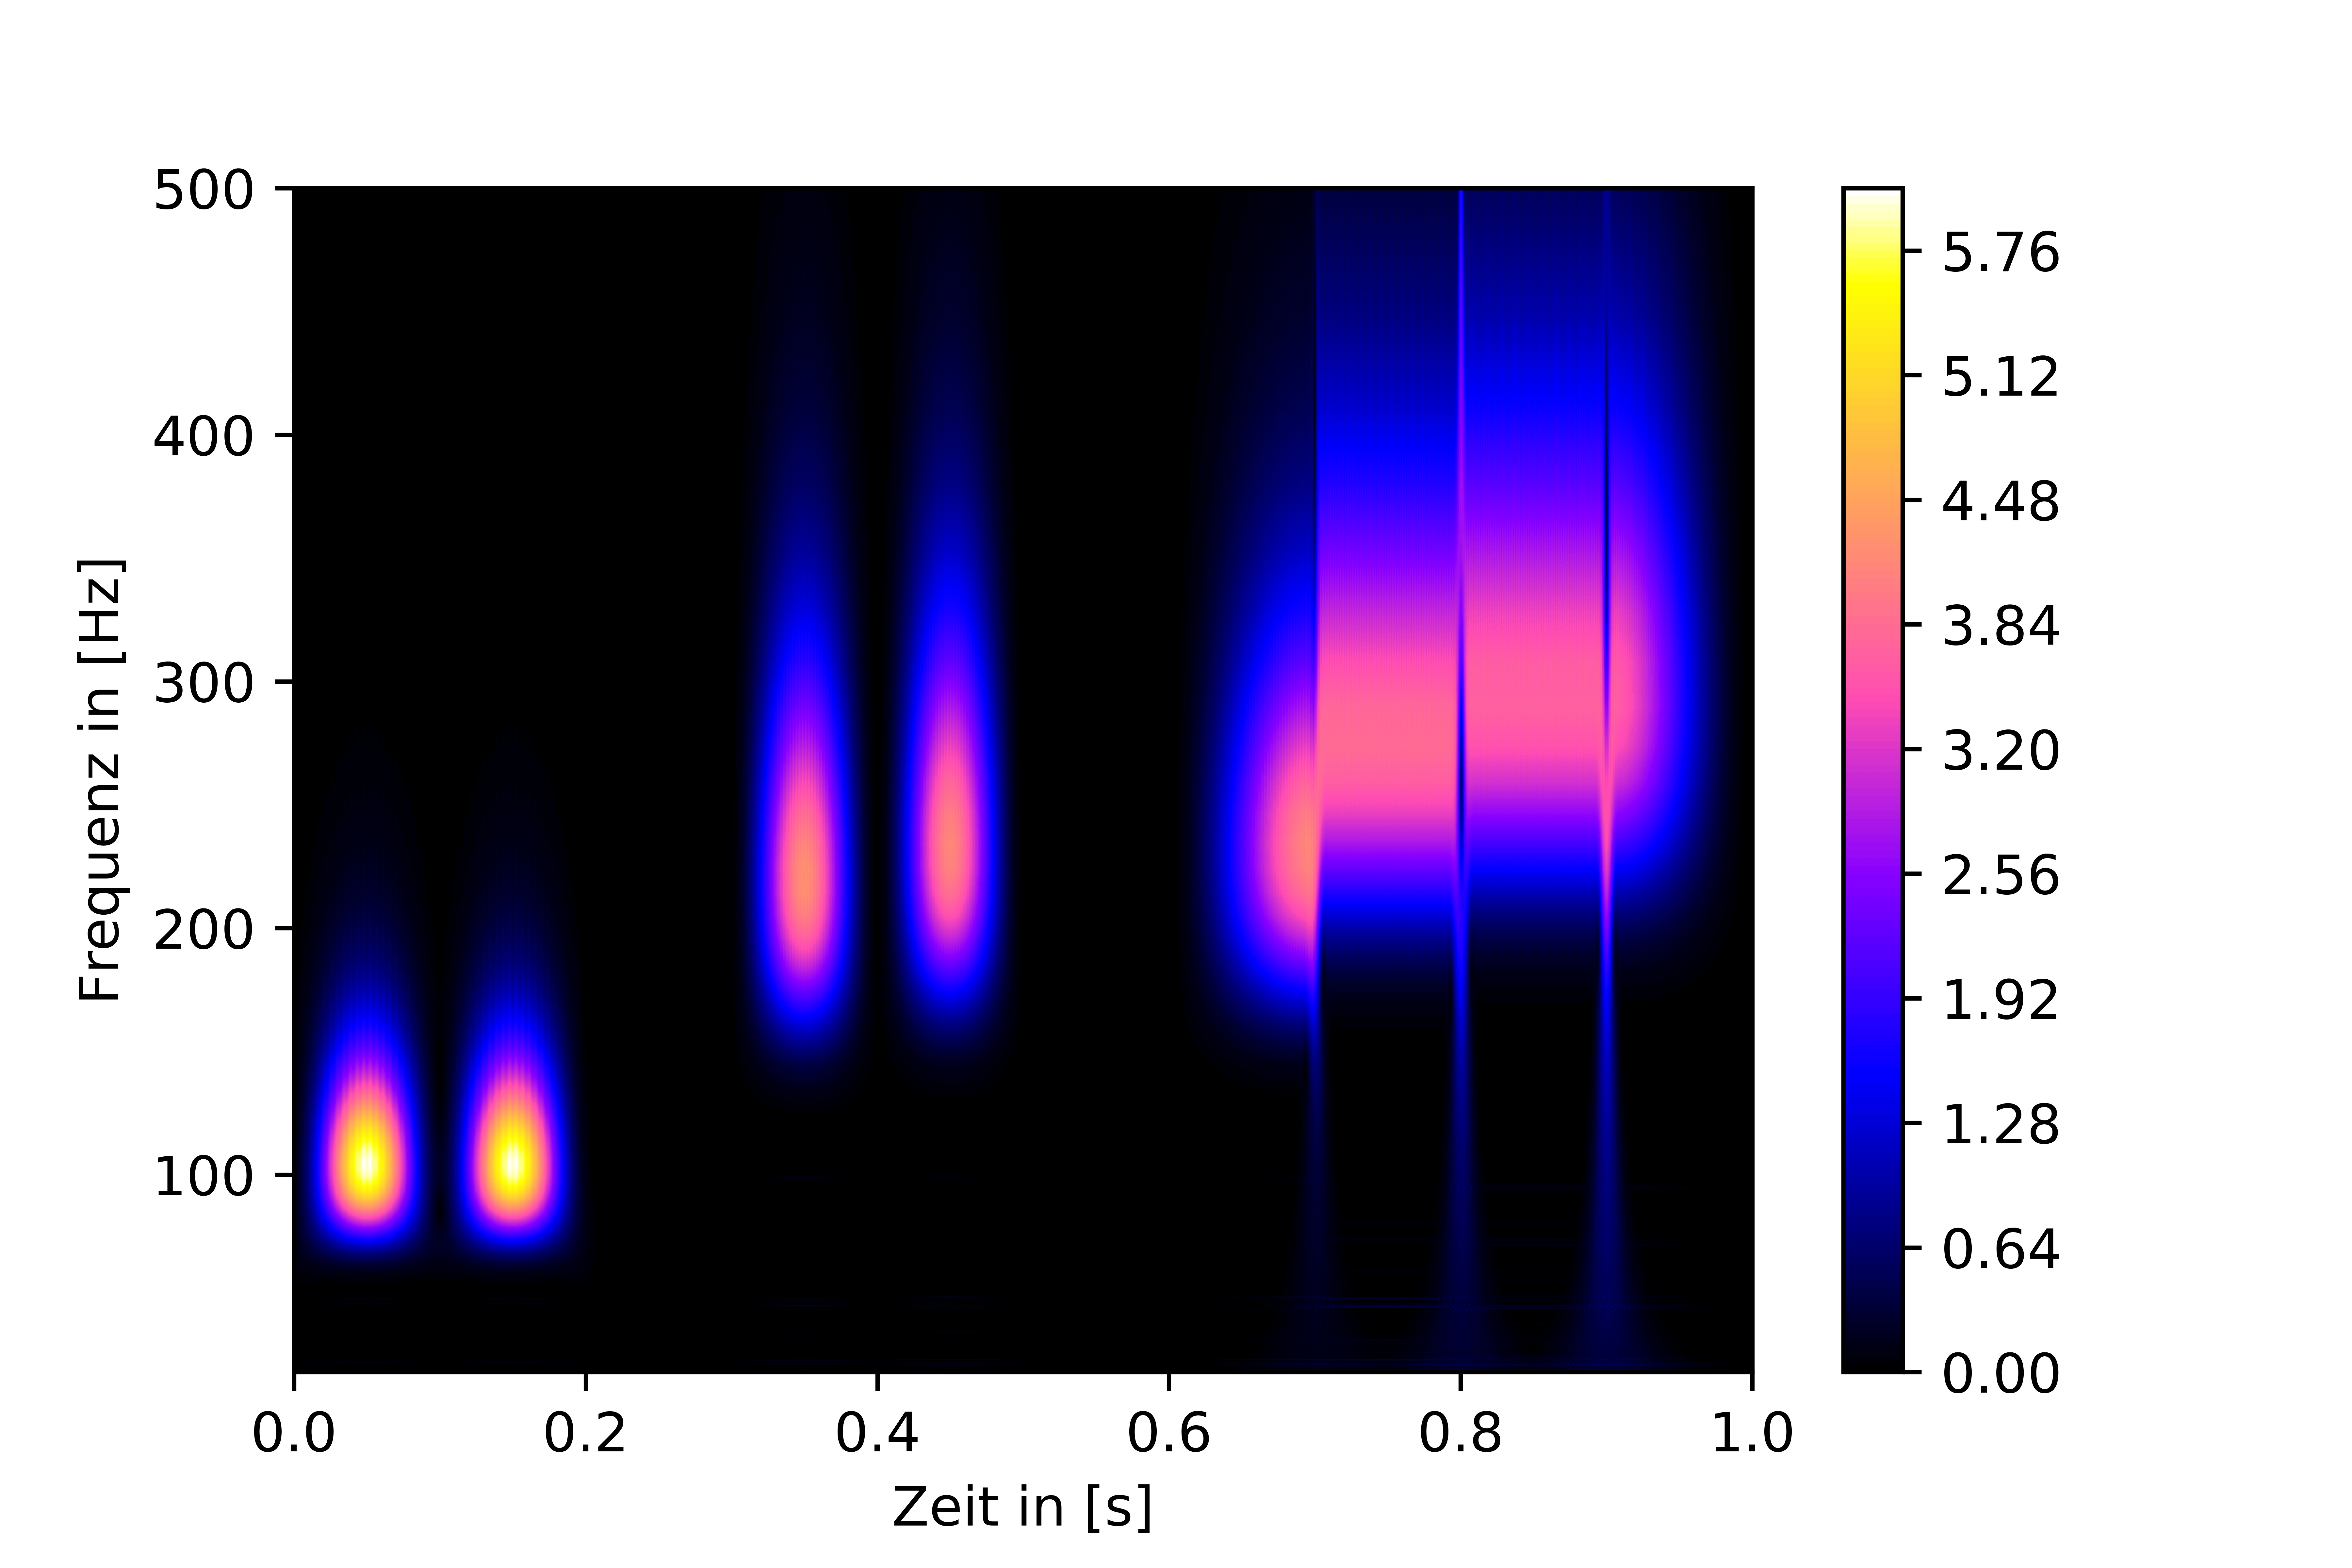
\includegraphics[width=1.3\linewidth]{papers/autotune/sections/frames/images/cwt.jpg}
		\captionof{figure}{Cwt Analyse mit komplexem Gauss Wavelet des Testsignal}\label{fig:stft256}
		&   \includegraphics[width=1.3\linewidth]{papers/autotune/sections/frames/images/12dwt.jpg}   
		\captionof{figure}{Dauberchi 8 Frame Analyse des Testsignal}\label{fig:cwtsweep}         
	\end{tabularx}
	\caption{Vergleich der Absolutwerte von der cwt und der Frame Analyse mit 12 Basen}
	\label{fig:Frame-Analyse}
\end{figure}%



\begin{figure}[!ht]
	\begin{minipage}{.5\linewidth}
		\includegraphics[width=\linewidth]{papers/autotune/sections/frames/images/1dwt.jpg}
		\caption{Frame-msa mit 1 Basis}
	\end{minipage}%

	
	\begin{minipage}{.5\linewidth}
	\centering
	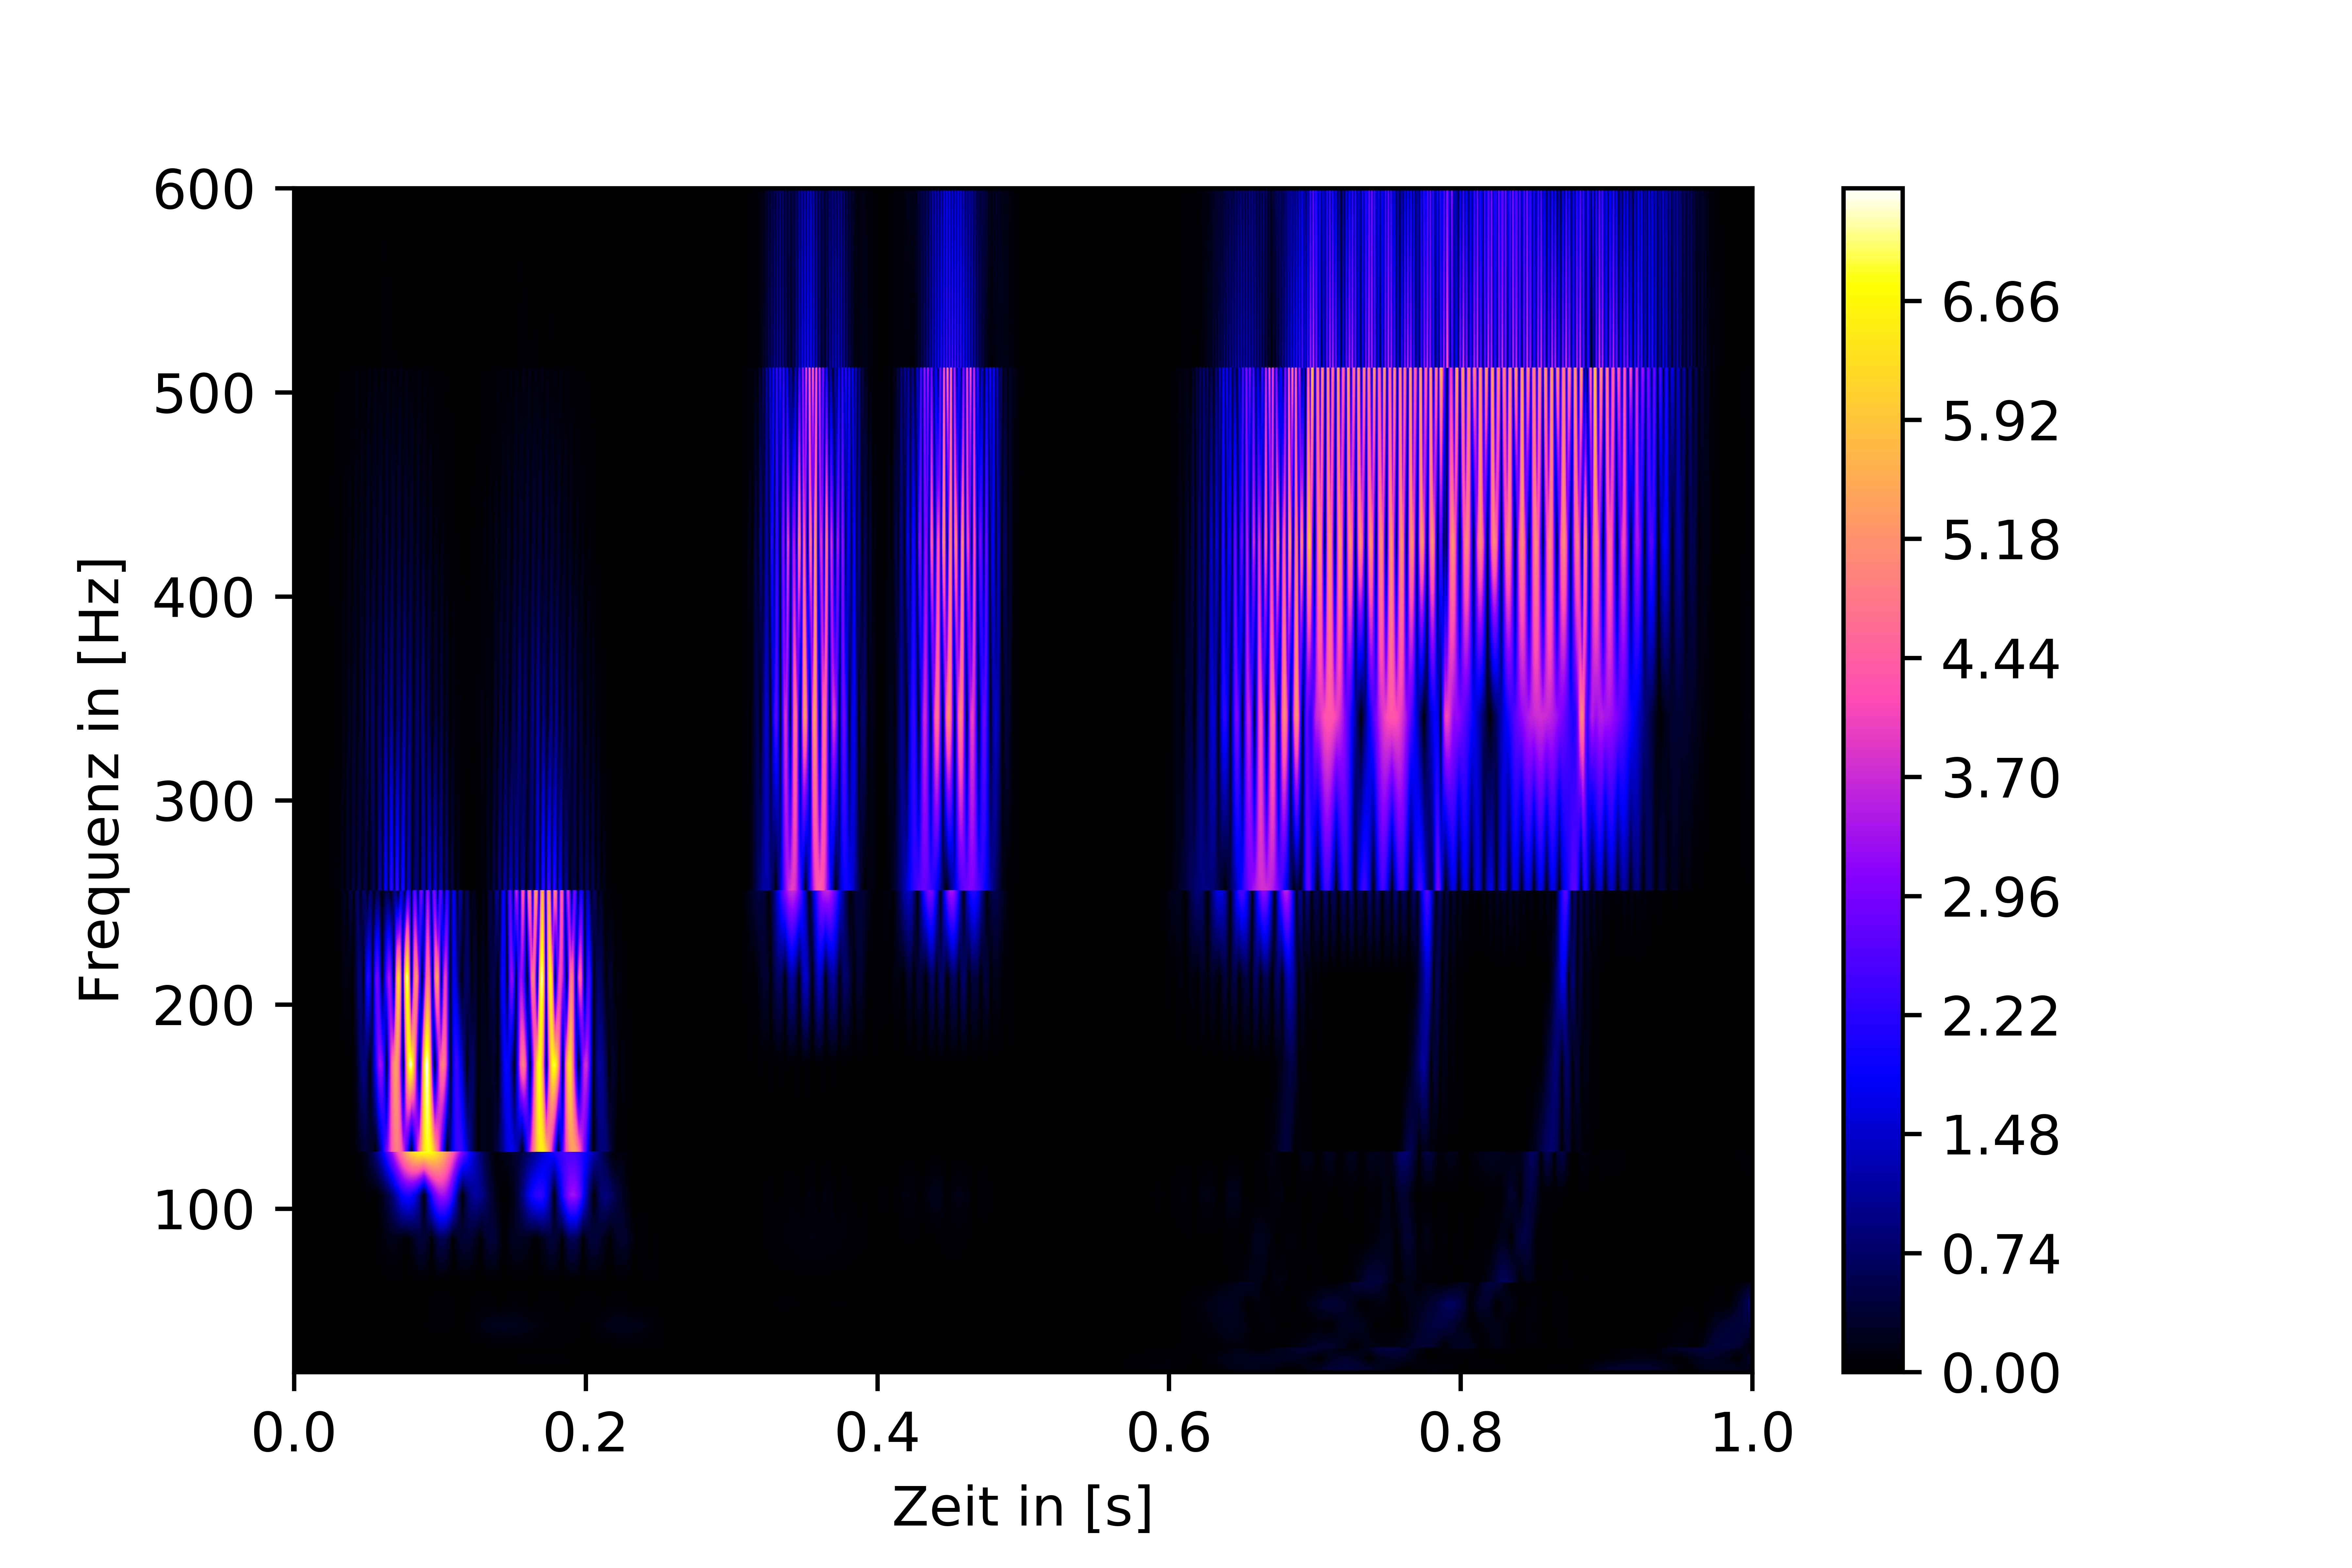
\includegraphics[width=\linewidth]{papers/autotune/sections/frames/images/4dwt.jpg}
	\caption{Frame-msa mit 4 Basen}
	\end{minipage}

	\begin{minipage}{.5\linewidth}
	\centering
	\includegraphics[width=\linewidth]{papers/autotune/sections/frames/images/12dwt.jpg}
	\caption{Frame-msa mit 12 Basen}
	\end{minipage}
	
	\begin{minipage}{.5\linewidth}
		\centering
		\includegraphics[width=\linewidth]{papers/autotune/sections/frames/images/24dwt.jpg}
		\caption{Frame-msa mit 24 Basen}
	\end{minipage}

	
	\caption{Verschiedene Fensterfunktionen und deren Beschreibung}\cite{wikipedia:Window}
	\label{fig:STFTtab}
\end{figure}


Von diesen Analyseresultaten sollen nun auch die Frequenzen extrahiert werden. Dabei macht man sich die Lokalen maximas der Matrix zunutze. Man vergleicht in der Matrix selber die jeweiligen nachbar Werte ob der Wert grösser oder kleiner ist. Von den Lokalen maximas werden die Koordinaten gesammelt welche dann mit den Level verglichen werden kann und so die Frequenz gefunden.\\
Um eine gute Qualität von Peak zu erhalten wurde noch ein Maximum Filter auf die Matrix angewendet. Dieser ersetzt in dem vordefinierten radius $r$ die Werte einer Matrix mit den Lokal gefundenen Maximalwert. Das Ziel des Maximum Filters ist die elimination der Nullstellen die direkt in den wichtigen Signalverläufen vorkommen. Durch dieser Maximal Filter werden jedoch auch Resultate verfälscht, was in den Versuchen gerade im Frequenzbereich sichtbar wurde. Dieser ist mit der relativ beschränkten Ahnzahl Level und Basen, viel empfindlicher auf Störungen, als die sehr fein aufgelöste Zeitachse. \\
In der Folgenden Grafik\ref{fig:cwt_max} wurde das genannte Ferfahren um Maximalstellen zu finden an der cwt Analyse angewendet. Diese kann somit als Referenz dienen. 

\begin{figure}[!ht]
	\centering
	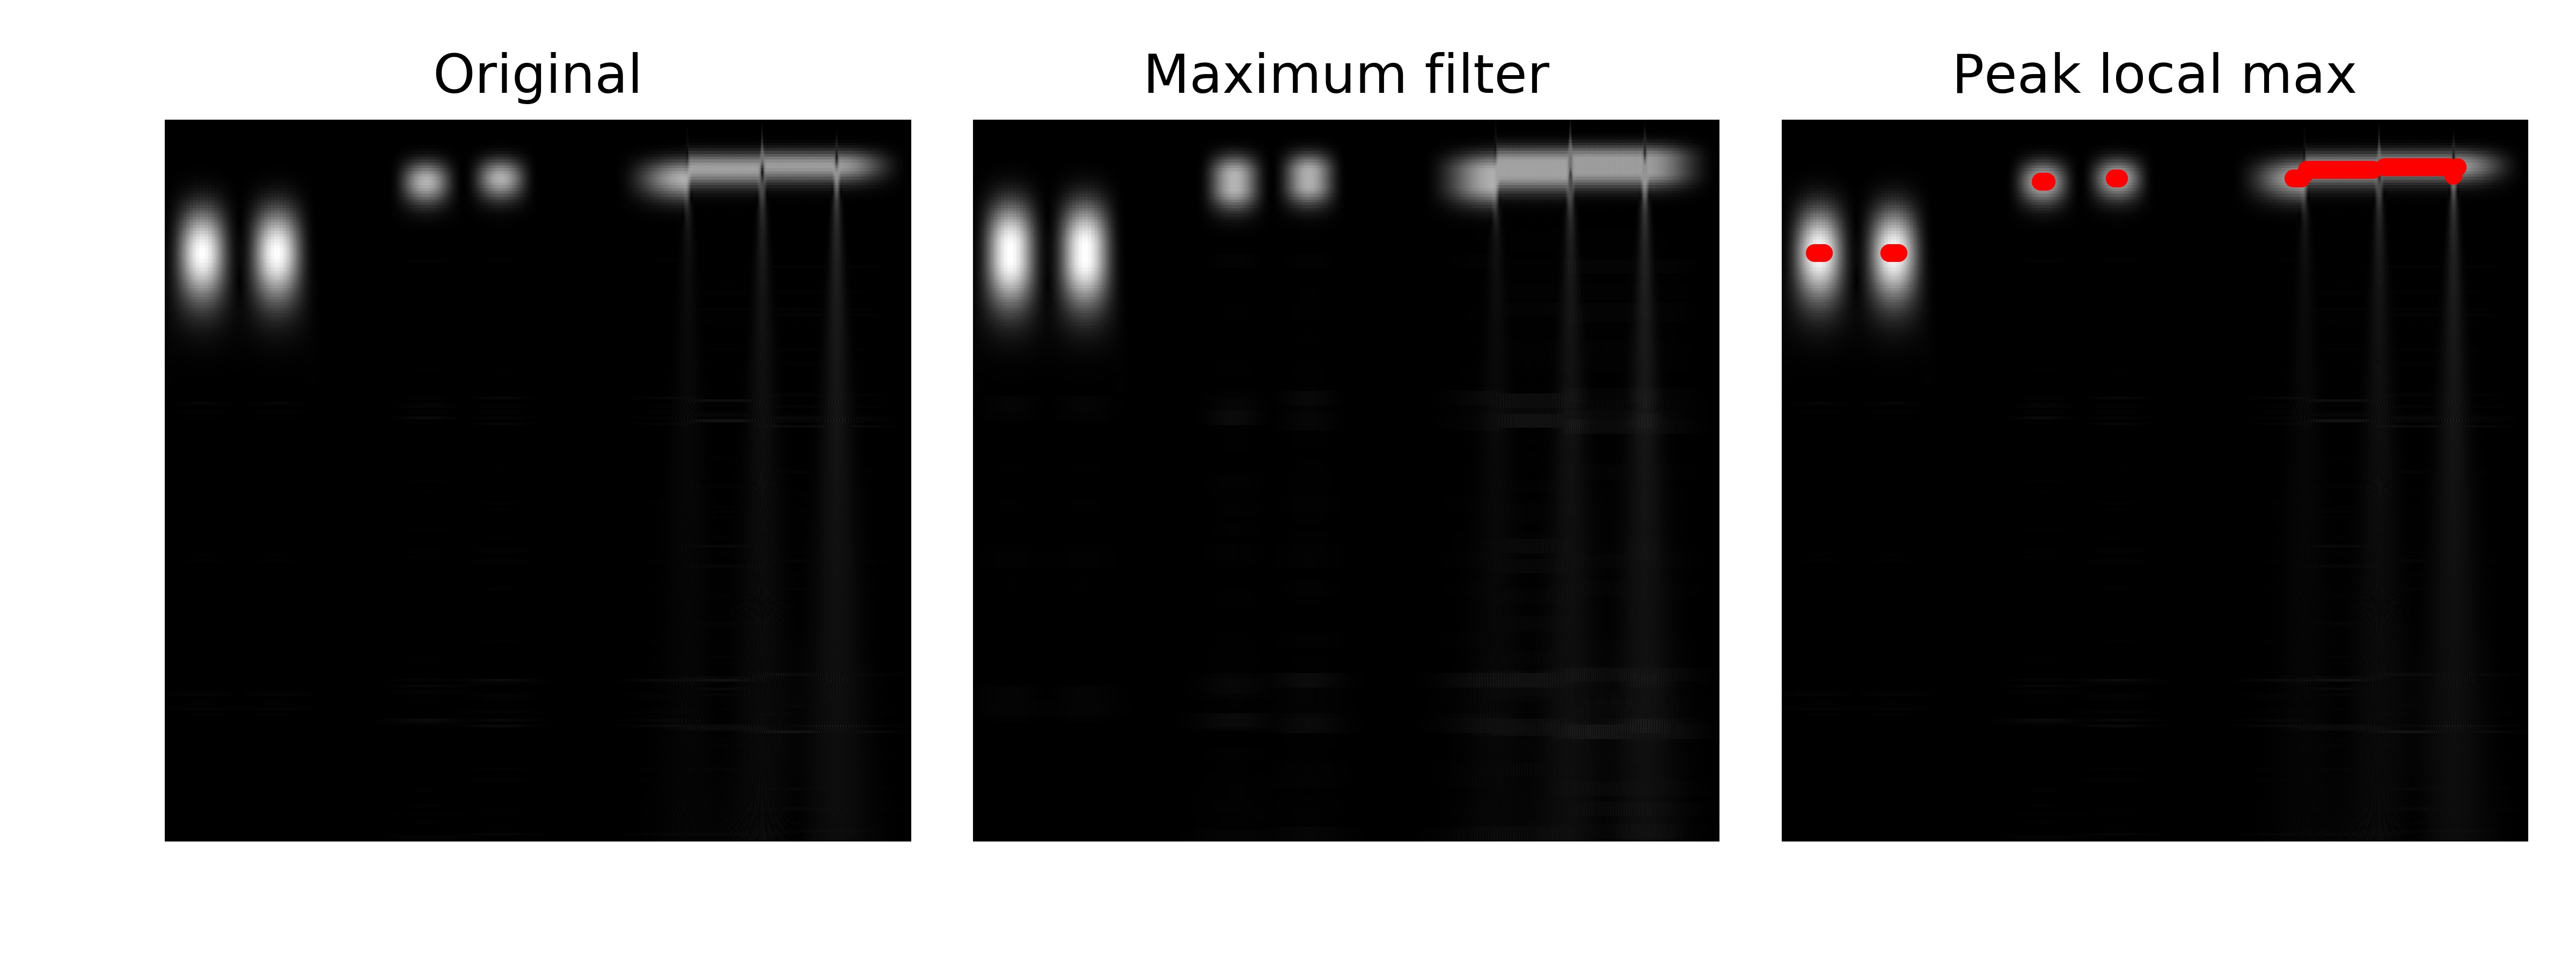
\includegraphics[width=\linewidth]{papers/autotune/sections/frames/images/cwtmaxima.jpg}
	\captionof{figure}{Maxima berechnung  des cwt}\label{fig:cwt_max}
\end{figure}%
In der cwt Grafik sieht man schön wie stabil die Frequenzen in der jeweils konstanten Frequenz angezeigt wird. Auch wenn man das Ergebnis der Koordinaten zurück rechnet kommt man auf die richtigen Frequenzen. Sprünge, Anfangswerte und jegliche andere Unstetigkeit der Funktion verzeiht auch die Ergebnisse der cwt.
\\
Die nächste Grafik \ref{fig:msa_max} bildet die Frame-msa ab, welche nach der fleichen Art wie \ref{fig:cwt_max} Analysiert wurde. Man bekommt die Frequenz nicht 
\begin{figure}[!ht]
	\centering
	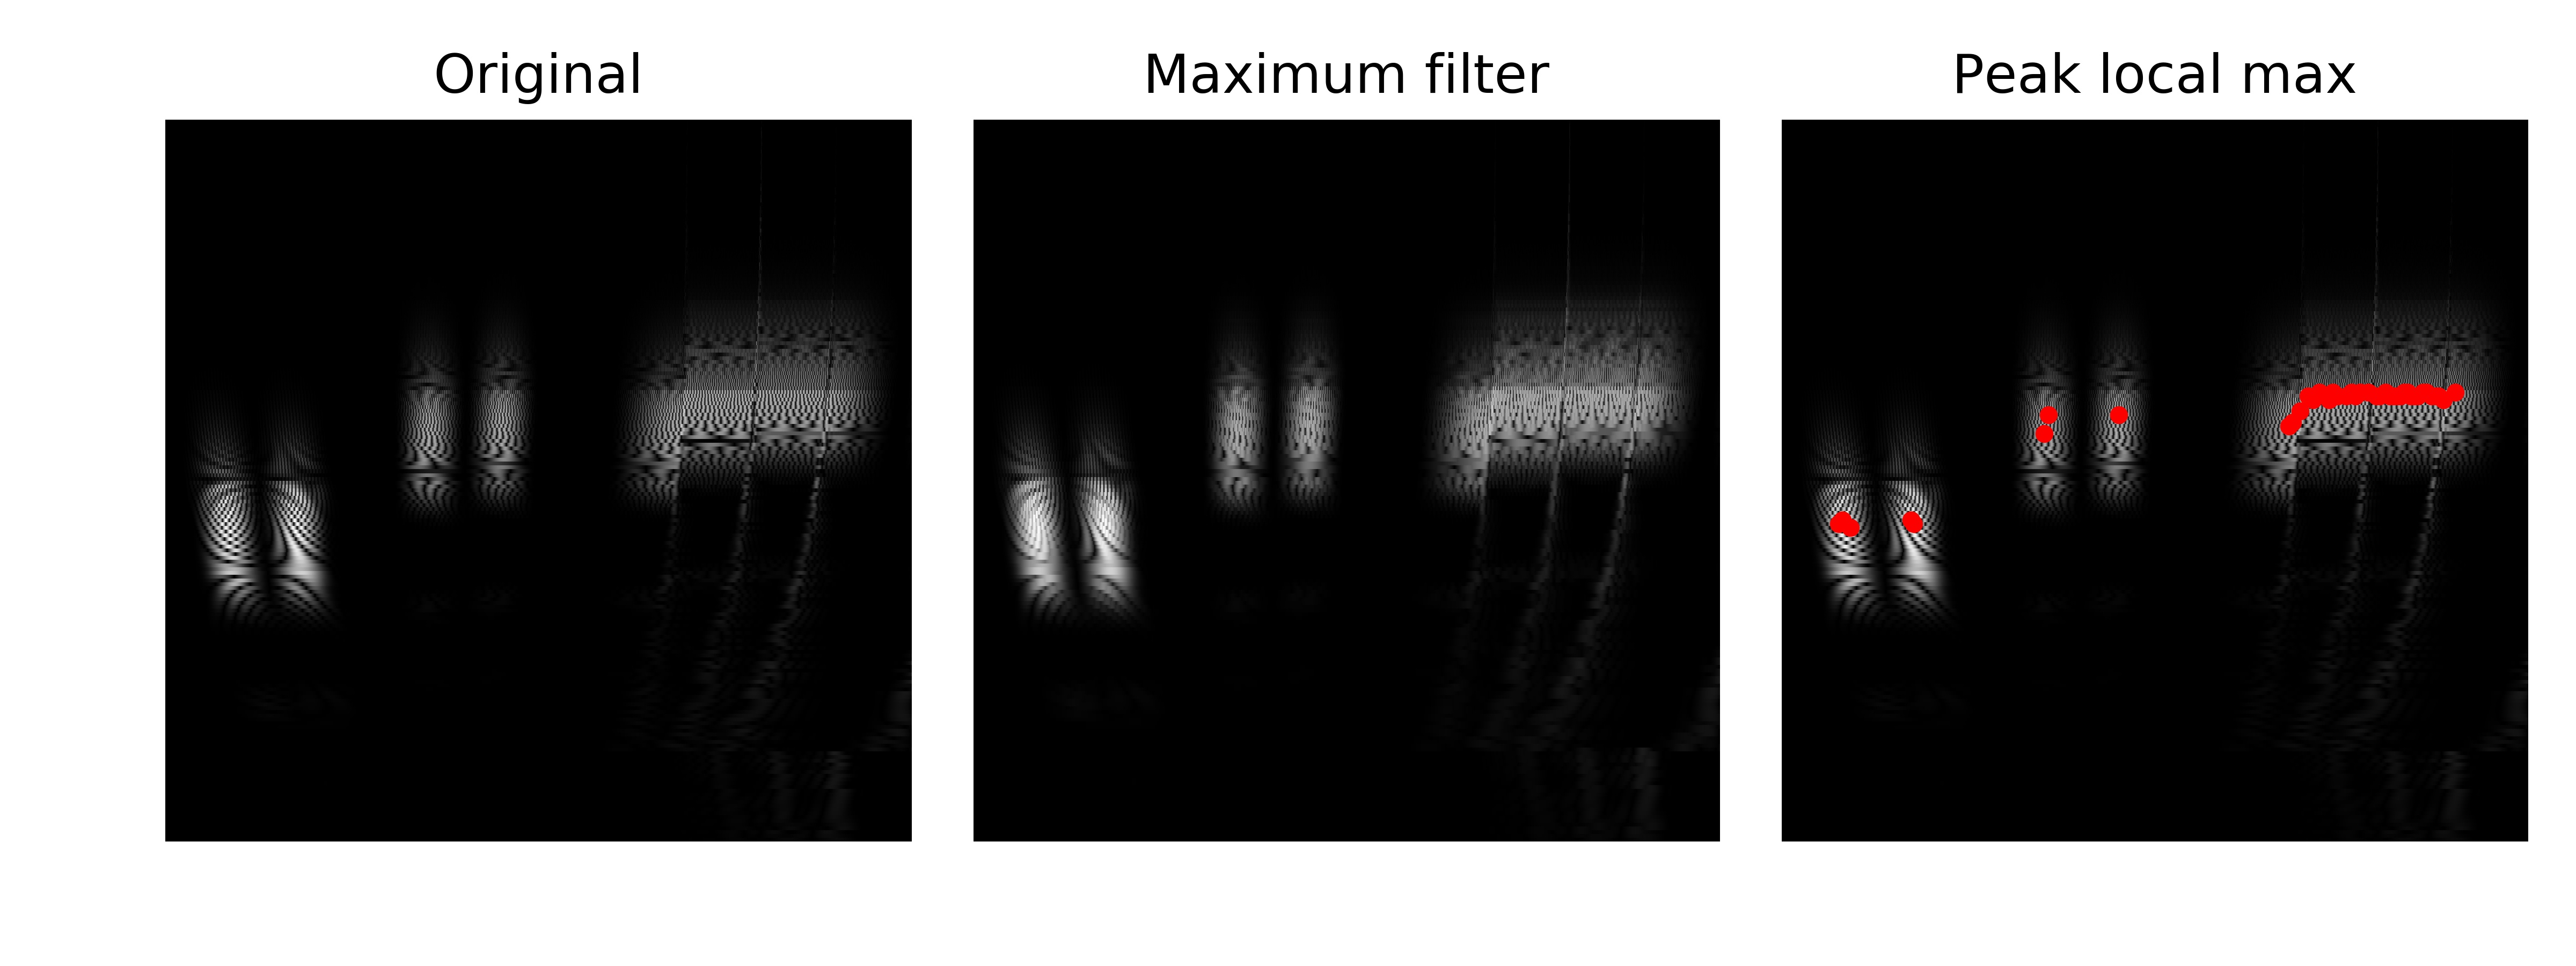
\includegraphics[width=\linewidth]{papers/autotune/sections/frames/images/dwtmaxima.jpg}
	\captionof{figure}{Maxima berechnung  der Frame-msa}\label{fig:msa_max}
\end{figure}%


